\documentclass[11pt,a4paper]{article}

\usepackage[margin=1in]{geometry}
\usepackage{amsmath,amssymb}
\usepackage{booktabs}
\usepackage{tabularx}
\usepackage{array}
\usepackage{longtable}
\usepackage{graphicx}
\usepackage{hyperref}
\usepackage{enumitem}
\usepackage{microtype}

\hypersetup{
  colorlinks=true,
  linkcolor=black,
  citecolor=black,
  urlcolor=blue
}

\setlist[itemize]{leftmargin=1.5em}
\setlist[enumerate]{leftmargin=1.5em}
\renewcommand{\arraystretch}{1.15}

\title{Defect Detection Technology for Multi-Material Surfaces Based on 3D Focus-Stack Reconstruction and Deep Learning}
\author{Li Shenshi \and Qian Fengfan}
\date{Zhejiang University SRTP Final Project Paper\\May 2026}

\begin{document}

\maketitle

\begin{abstract}
Multi-material surface defect inspection requires both two-dimensional texture information and three-dimensional morphology. In precision manufacturing, additive manufacturing, metal surface processing, micro-hole machining and optoelectronic packaging, defects such as dents, scratches, burrs, steps, collapsed hole edges and local roughness changes are often expressed as geometric variations rather than simple grayscale anomalies. Depth from Focus (DFF) is an interpretable and low-cost route for recovering relative 3D shape from a focus stack, but traditional DFF is sensitive to glare, low texture, periodic patterns and multi-peak focus responses.

This paper presents a relative 3D reconstruction and defect morphology visualization pipeline for multi-material surfaces. The pipeline includes Original DFF, post-processed DFF, Glare-Aware DFF (GADFF), adaptive traditional baselines inspired by Lee et al. and Li et al., and three learning-based correction models: TinyDepthNet, Focus-ResUNet and a prior-anchored residual Focus-ResUNet variant. Synthetic focus-stack samples with ground-truth height maps are generated for quantitative evaluation, while real focus-stack samples are used for engineering verification and relative morphology visualization.

Experiments on seven synthetic test samples show that Focus-ResUNet achieves the lowest average MAE of \(53.22~\mu\mathrm{m}\), outperforming Original DFF with \(100.55~\mu\mathrm{m}\) and TinyDepthNet with \(57.31~\mu\mathrm{m}\). The improvement is especially clear on the P10 V-valley sample, where Focus-ResUNet reduces MAE from \(160.17~\mu\mathrm{m}\) for Original DFF to \(62.07~\mu\mathrm{m}\). On real samples without calibrated height ground truth, TinyDepthNet gives the most stable visual reconstruction, with the lowest average roughness of 0.0067 and far fewer low-confidence spikes than traditional DFF methods. These results form two complementary evidence chains: quantitative validation on synthetic samples with ground truth and relative morphology verification on real samples.
\end{abstract}

\noindent\textbf{Keywords:} multi-material surface; defect morphology characterization; Depth from Focus; focus stack; relative 3D reconstruction; glare-aware DFF; Focus-ResUNet; deep learning

\section{Introduction}

Surface defects directly affect fatigue life, assembly accuracy, contact reliability and product appearance. In industrial inspection, a defect may not appear as a simple bright or dark region in a two-dimensional image. A dent, scratch, burr, local step, collapsed hole edge or roughness variation can have a weak intensity signature but a clear three-dimensional morphology. A reliable inspection pipeline therefore needs to recover not only the texture image but also the local shape of the surface.

Several methods can measure surface morphology, including contact profilometry, confocal microscopy, white-light interferometry, structured light, binocular vision and Shape from Focus or Depth from Focus. Among them, focus-stack based DFF is attractive because it reuses a sequence of images captured at different focal planes. For each pixel, the method computes a focus measure across the stack and maps the layer with the strongest focus response to a relative depth or height. Compared with high-end metrology equipment, DFF is easier to reproduce with ordinary microscope imaging systems and gives an interpretable computational path.

However, multi-material surfaces introduce serious reconstruction challenges. In this project, ``multi-material surface'' refers to different surface imaging conditions caused by material reflectance, texture density, roughness and defect morphology. It is not treated as a material classification task. Metallic surfaces may produce specular highlights, saturation and stray-light-like responses. 3D-printed surfaces often contain layered manufacturing texture and diffuse roughness. Key-texture samples and hole edges contain dense directional patterns and sharp discontinuities. Low-texture or high-glare regions may create unstable multi-peak focus responses. Under these conditions, traditional DFF can select a false focal layer and produce isolated height spikes, broken edges or distorted morphology.

The project is therefore framed as relative 3D reconstruction and defect morphology visualization for multi-material surface focus stacks. Real samples are used to verify that the pipeline can run on practical focus stacks and generate plausible relative height maps. Synthetic samples, which provide ground-truth height maps, are used for quantitative algorithm comparison. This distinction is important: synthetic samples support MAE-based accuracy claims, while real samples without external height calibration support only relative morphology and stability analysis.

The main contributions are as follows:
\begin{enumerate}
  \item A reproducible relative 3D reconstruction workflow is built for multi-material focus stacks, covering Original DFF, post-processed DFF, GADFF, two adaptive traditional baselines and three learning-based models.
  \item A synthetic focus-stack dataset with known height maps is constructed for quantitative comparison under controlled geometry, texture and reflectance conditions.
  \item Focus-ResUNet combines 17 focus-stack frames, 16 adjacent focal-difference channels and five DFF/GADFF prior channels, and achieves the lowest average MAE on the seven synthetic test samples.
  \item Real focus-stack samples are reconstructed with multiple algorithms and evaluated using no-reference stability indicators such as roughness, edge correlation, relative dynamic range and low-confidence spike count.
  \item The work separates two evidence chains: Focus-ResUNet is the strongest model under synthetic ground-truth evaluation, while TinyDepthNet gives the most stable visualization on current real samples.
\end{enumerate}

\section{Related Work}

\subsection{Focus-measure based 3D shape recovery}

Shape from Focus and Depth from Focus rely on the observation that an object point appears sharper when it lies near the optical focal plane and becomes blurred when it moves away from focus. By computing a focus measure for each layer in a focus stack, the best-focused layer can be used to estimate relative depth. Early work by Nayar and Nakagawa established the feasibility of 3D shape recovery from focus. Later studies compared focus-measure operators such as gradient, Laplacian, variance and frequency-domain responses.

The focus-measure operator has a direct influence on reconstruction stability. Gradient-based operators are sensitive to edges and texture, while Laplacian operators emphasize local high-frequency sharpness and can amplify noise. This project uses a combination of Laplacian response and Tenengrad gradient response as the Original DFF baseline, balancing local sharpness and edge strength.

\subsection{Adaptive window and iterative traditional methods}

Traditional DFF usually computes or smooths focus responses within a local support window. A small window preserves details but is sensitive to noise and weak texture. A large window improves stability but can smooth holes, steps and small defects. Lee et al. proposed adaptive window selection for 3D shape recovery from image focus, adjusting the support size according to local structure. Li et al. further proposed adaptive window iteration to enhance focus-based shape recovery.

In this project, the core ideas of these methods are implemented as lightweight baselines adapted to the 17-frame focus stacks. They are used to compare the proposed learning-based models against stronger traditional references rather than only against a simple fixed-window DFF baseline.

\subsection{Deep depth from focus and focal-difference features}

Deep learning can learn nonlinear correction patterns from simulated or calibrated data. For DFF, the network can use not only spatial image texture but also the response variation along the optical axis. Yang et al. proposed Deep Depth from Focus with Differential Focus Volume, showing that adjacent focal differences provide useful depth cues. This idea motivates Focus-ResUNet in this project.

Focus-ResUNet is an engineering adaptation rather than a direct reproduction of the full original DFV model. It uses 17 original focus-stack frames, 16 adjacent focal-difference channels and five DFF/GADFF prior channels. This design keeps the physical information from traditional DFF and allows the network to learn where to trust the traditional prior and where to correct it.

\subsection{Zoom microscopy and defect inspection}

Zoom-microscopy based 3D measurement is relevant to microstructure inspection, surface roughness analysis and industrial defect detection. Existing Chinese reviews and measurement studies indicate that focus-stack acquisition, focus evaluation, noise suppression, step size and surface reflectance jointly affect final 3D measurement. This project follows that engineering view: DFF reconstruction is not only an algorithmic problem, but a pipeline involving imaging, focus response, prior modeling, post-processing and learning-based correction.

\section{Samples and Evaluation Protocol}

\subsection{Real focus-stack samples}

The real focus-stack samples include 3D printing layer texture, 3D printed surface, metallic dent or hole samples, key-texture samples, circular-hole samples, key-tip samples and the 1124 sample. These samples cover different imaging conditions. The 3D-printed samples represent layered and rough diffuse surfaces. Metallic dent, key-texture and key-tip samples represent specular reflection, fine directional texture and sharp local edges. Circular-hole and micro-hole samples represent regular hole boundaries and low-texture inner regions.

The real samples do not have synchronized ground-truth height maps from a profilometer, white-light interferometer, confocal microscope or calibrated step standard. Therefore, they are used for relative 3D reconstruction, focus confidence analysis, dynamic-range observation and visual stability comparison. Their height maps should not be interpreted as absolute micrometer measurements.

\begin{table}[htbp]
\centering
\caption{Real focus-stack samples and imaging challenges.}
\small
\begin{tabularx}{\textwidth}{p{0.20\textwidth}p{0.23\textwidth}p{0.27\textwidth}X}
\toprule
Real sample type & Surface property & Main imaging challenge & Role in this paper \\
\midrule
3D printing layer texture & Additive manufacturing texture & Periodic layers, rough diffuse reflection & Verify continuity of layered morphology \\
3D printed surface & Rough manufactured surface & Low-texture regions mixed with roughness & Evaluate smoothing-detail balance \\
Metallic dent or hole & Reflective metal with local concavity & Specular highlights and abrupt hole edges & Test reconstruction under strong reflection \\
Key texture & Dense metallic texture & Directional fine texture and local highlights & Test stability on fine texture \\
Circular or micro hole & Regular hole boundary & Sharp boundary and low-texture interior & Test edge preservation \\
Key tip & Sharp metallic edge & Tip highlight, occlusion and height jump & Test abrupt-structure visualization \\
1124 sample & Supplementary real sample & Mixed morphology and reflectance & Verify general workflow operation \\
\bottomrule
\end{tabularx}
\end{table}

\subsection{Synthetic focus-stack samples}

Synthetic samples are generated to provide ground-truth height maps for quantitative evaluation. The test set includes seven representative surfaces: P10 V-valley with a rough wide bottom, A-type ridge with Perlin roughness, fractal mountain, Perlin ridge, Perlin step, periodic stripe roughness and composite corrosion pits. These samples cover roughness, texture frequency, reflectance risk and defect morphology.

The synthetic generation pipeline follows a geometry-rendering-defocus structure. A height field \(Z(x,y)\) is first generated. Surface gradients are used to estimate normal direction, and the normal z-component approximates coaxial illumination and observation consistency. Base intensity is formed by low-frequency albedo and diffuse reflection. Specular highlights are controlled by roughness, base specular coefficient and surface normal. Strong highlight regions are diffused to simulate bloom-like glare, with low-frequency stray light and ghost flare added to interfere with focus evaluation.

Each synthetic sample contains 17 focus-stack frames. The focal planes cover the height range of the sample. The project follows a consistent depth-direction convention: the first frame corresponds to the higher focal plane, and normalized height is mapped as
\begin{equation}
D = 1 - \frac{k}{N-1}.
\end{equation}

Layer-wise glare, stray light, PRNU, row-column bias, shot noise, read noise and 8-bit quantization are added. A glare-risk map is generated from near-saturated highlights, local bright anomalies, stray light and bloom regions, and is used both as an interpretable prior and as an input channel for learning models.

\begin{table}[htbp]
\centering
\caption{Synthetic test samples.}
\small
\begin{tabularx}{\textwidth}{p{0.30\textwidth}Xp{0.16\textwidth}p{0.16\textwidth}}
\toprule
Test sample & Structure and texture & Resolution & Height range \\
\midrule
P10 V-valley with rough wide bottom & Wide valley, rough bottom, reflectance risk & \(960 \times 540\) & \(1200~\mu\mathrm{m}\) \\
A-type ridge with Perlin roughness & Protruding ridge, Perlin roughness & \(960 \times 540\) & \(1280~\mu\mathrm{m}\) \\
Fractal mountain & Mountain structure, fractal roughness & \(640 \times 360\) & \(1100~\mu\mathrm{m}\) \\
Perlin ridge & Ridge structure, Perlin roughness & \(640 \times 360\) & \(1020~\mu\mathrm{m}\) \\
Perlin step & Step structure, Perlin roughness & \(640 \times 360\) & \(1040~\mu\mathrm{m}\) \\
Periodic stripe roughness & Periodic texture, stripe roughness & \(640 \times 360\) & \(920~\mu\mathrm{m}\) \\
Composite corrosion pits & Multi-scale pits and grooves & \(960 \times 540\) & \(1420~\mu\mathrm{m}\) \\
\bottomrule
\end{tabularx}
\end{table}

The original synthetic dataset contains 12 training samples, 5 validation samples and 7 fixed test samples. After adding reflectance-augmented cases during training and validation, the learning models use 27 training samples, 10 validation samples and the same 7 fixed test samples. All reported test conclusions come from samples excluded from training.

\subsection{Metrics}

For synthetic samples, the main metric is mean absolute error:
\begin{equation}
\mathrm{MAE}=\frac{1}{|\Omega|}\sum_{p\in\Omega}|\hat{H}(p)-H(p)|.
\end{equation}

High-risk-region MAE is computed in regions with high glare or reflectance risk. Edge-region MAE is computed in regions with large ground-truth height gradients. These two regional metrics evaluate whether a method handles strong reflection and structural boundaries.

For real samples, no-reference metrics are used because calibrated height truth is unavailable. The main indicators are relative dynamic range, roughness, edge correlation and low-confidence spike count. Roughness measures local height oscillation. Relative dynamic range measures whether output height is over-amplified or over-smoothed. Edge correlation compares reconstructed height edges with image edges. Low-confidence spike count estimates isolated pseudo-peaks in unreliable focus regions.

\section{Methods}

\subsection{Original DFF}

Given a focus stack \(\{I_1,I_2,\ldots,I_N\}\), Original DFF computes a focus response \(F_i\) for each frame. This project combines Laplacian response and Tenengrad gradient response. The best focal layer at each pixel is selected by
\begin{equation}
k^*(p)=\arg\max_i F_i(p).
\end{equation}

The selected focal index is then mapped to normalized relative height:
\begin{equation}
D(p)=1-\frac{k^*(p)-1}{N-1}.
\end{equation}

Original DFF is training-free, interpretable and directly applicable to real focus stacks. Its main weakness is sensitivity to noise, glare, low texture and multi-peak focus responses.

\subsection{Post-processed DFF and Glare-Aware DFF}

Original DFF + post applies median filtering, Gaussian smoothing and morphological opening to the raw height map. This improves visual stability and suppresses isolated spikes, but it may also smooth fine geometry.

GADFF models highlight and glare risk. Let \(R(p,i)\) denote the glare risk of pixel \(p\) in layer \(i\). The focus response is down-weighted as
\begin{equation}
\tilde{F}_i(p)=F_i(p)(1-\lambda R(p,i)),
\end{equation}
where \(\lambda\) controls risk suppression. GADFF is useful because it converts strong-reflection interference into an explicit risk prior. However, as a standalone depth recovery rule, it can over-suppress valid edge responses when bright real structure is confused with glare. In this project, GADFF is therefore mainly used as an interpretable prior channel for learning-based models.

\subsection{Adaptive traditional baselines}

The Lee2013 adaptive-window baseline changes the local support window according to texture and structure. Larger windows are used in low-texture or flat regions to stabilize the response, while smaller windows are used near edges to reduce smoothing.

The Li2019 adaptive-iteration baseline adds iterative focus-response enhancement on top of adaptive windowing. It reduces isolated false focus layers and improves the smoothness of the focus curve. Both baselines are lightweight implementations of the original ideas and are evaluated under the same data and metrics as the proposed models.

\subsection{TinyDepthNet}

TinyDepthNet is a compact learning-based correction model. Its input contains the 17 focus-stack frames and five prior channels:
\begin{equation}
X_{\mathrm{tiny}}=\mathrm{concat}(I_1,\ldots,I_N,R,D_{\mathrm{DFF}},C_{\mathrm{DFF}},D_{\mathrm{GADFF}},C_{\mathrm{GADFF}}),
\end{equation}
where \(R\) is the glare-risk map, \(D_{\mathrm{DFF}}\) and \(C_{\mathrm{DFF}}\) are DFF depth and confidence, and \(D_{\mathrm{GADFF}}\) and \(C_{\mathrm{GADFF}}\) are GADFF depth and confidence. The model predicts a normalized relative height map using a sigmoid-constrained output.

TinyDepthNet is trained with SmoothL1 loss and an edge-consistency term. Its smaller capacity acts as implicit regularization. On synthetic data, it improves over traditional DFF. On real samples, its conservative and smoother output gives better visual stability.

\subsection{Focus-ResUNet}

Focus-ResUNet is the main learning-based model in this project. It uses three types of input:
\begin{enumerate}
  \item Seventeen original focus-stack frames.
  \item Sixteen adjacent focal-difference frames.
  \item Five DFF/GADFF prior channels.
\end{enumerate}

The adjacent focal difference is
\begin{equation}
\Delta I_i = I_{i+1}-I_i,\quad i=1,2,\ldots,N-1.
\end{equation}

The full input is
\begin{equation}
X_{\mathrm{focus}}=\mathrm{concat}(S,\Delta S,P),
\end{equation}
where \(S\) is the focus stack, \(\Delta S\) is the focal-difference volume and \(P\) is the prior-channel set. The network uses residual U-Net structure, multi-scale encoder-decoder processing, skip connections and group normalization. Its mixed loss includes data error, gradient consistency, curvature consistency, normal consistency and prior consistency.

The core advantage of Focus-ResUNet is that focal differences capture how sharpness changes along the optical axis. Combined with DFF and GADFF priors, the model can learn structured correction patterns in glare, low-texture and edge regions.

\subsection{Prior-anchored residual Focus-ResUNet}

The prior-anchored residual Focus-ResUNet variant, also referred to as PA-FRU in this paper, predicts a bounded correction over a traditional prior. Let \(D_0\) be the prior depth, \(\Delta D\) the learned residual and \(G\) a gating coefficient. The output is
\begin{equation}
\hat{D}=D_0+G\Delta D.
\end{equation}

The design aims to stay close to the DFF/GADFF prior where it is reliable and apply limited correction in difficult regions. It reduces over-correction risk, but it may also under-correct samples where the original DFF prior is already poor, such as the P10 V-valley and periodic stripe cases.

\section{Experiments and Results}

\subsection{Average results on synthetic samples}

The average metrics on the seven synthetic test samples are shown in Table~\ref{tab:synthetic_average}.

\begin{table}[htbp]
\centering
\caption{Average metrics on seven synthetic test samples.}
\label{tab:synthetic_average}
\small
\begin{tabular}{lccc}
\toprule
Method & Average MAE & High-risk MAE & Edge MAE \\
 & \((\mu\mathrm{m})\) & \((\mu\mathrm{m})\) & \((\mu\mathrm{m})\) \\
\midrule
Original DFF & 100.55 & 46.32 & 206.61 \\
Original DFF + post & 63.81 & 29.72 & 149.04 \\
Lee2013 adaptive window & 62.35 & 30.52 & 146.83 \\
Li2019 adaptive iteration & 62.95 & 31.24 & 145.33 \\
GADFF & 105.83 & 46.38 & 210.60 \\
TinyDepthNet & 57.31 & 42.63 & 89.10 \\
Focus-ResUNet & \textbf{53.22} & 40.14 & \textbf{86.68} \\
PA-FRU & 62.52 & 30.08 & 126.91 \\
\bottomrule
\end{tabular}
\end{table}

Original DFF has an average MAE of \(100.55~\mu\mathrm{m}\), indicating that direct maximum-focus layer selection is unstable on complex synthetic surfaces. Post-processing reduces MAE to \(63.81~\mu\mathrm{m}\), showing that spatial smoothing and spike suppression are useful. Lee2013 adaptive window and Li2019 adaptive iteration achieve \(62.35~\mu\mathrm{m}\) and \(62.95~\mu\mathrm{m}\), respectively, forming strong traditional baselines.

The learning-based models improve overall accuracy. TinyDepthNet reaches \(57.31~\mu\mathrm{m}\), proving that supervised correction can reduce DFF error. Focus-ResUNet obtains the best average MAE of \(53.22~\mu\mathrm{m}\) and the best edge-region MAE of \(86.68~\mu\mathrm{m}\). This confirms the value of combining focal-difference features with DFF/GADFF priors. PA-FRU reaches \(62.52~\mu\mathrm{m}\). Its conservative prior anchoring is useful in some samples but limits correction in difficult cases.

GADFF alone has an average MAE of \(105.83~\mu\mathrm{m}\), slightly worse than Original DFF. This result does not invalidate glare modeling; it shows that hand-crafted glare down-weighting is insufficient as a standalone depth rule. Its main value is as an interpretable prior supplied to learning models.

\begin{figure}[htbp]
\centering
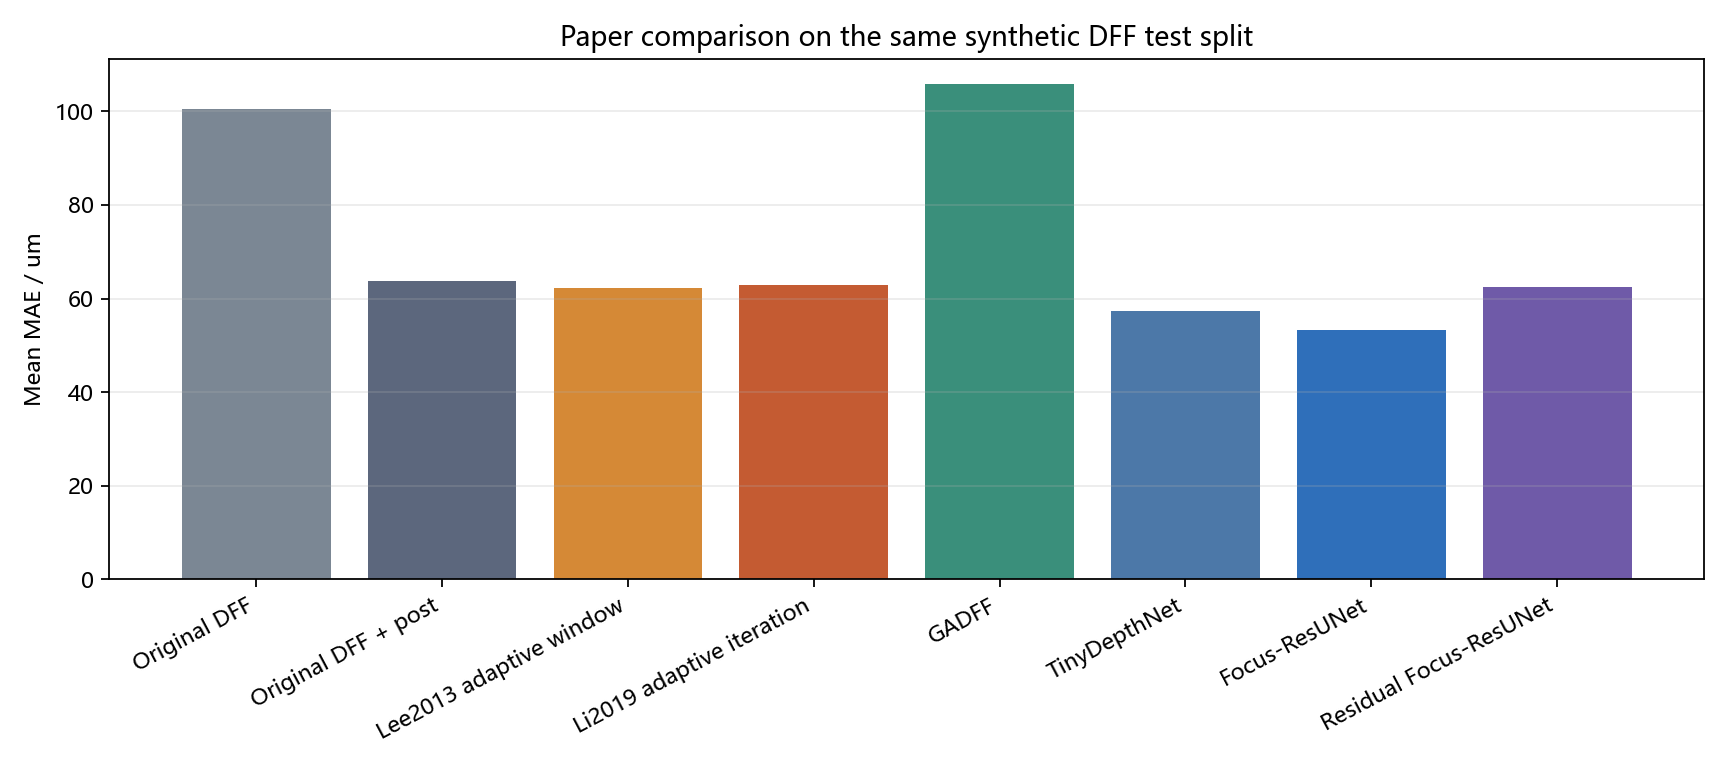
\includegraphics[width=0.86\textwidth]{results/figures/paper_comparison_mean_mae.png}
\caption{Average MAE comparison on the synthetic test set. Focus-ResUNet achieves the lowest mean error among the compared methods.}
\label{fig:mean_mae}
\end{figure}

\begin{figure}[htbp]
\centering
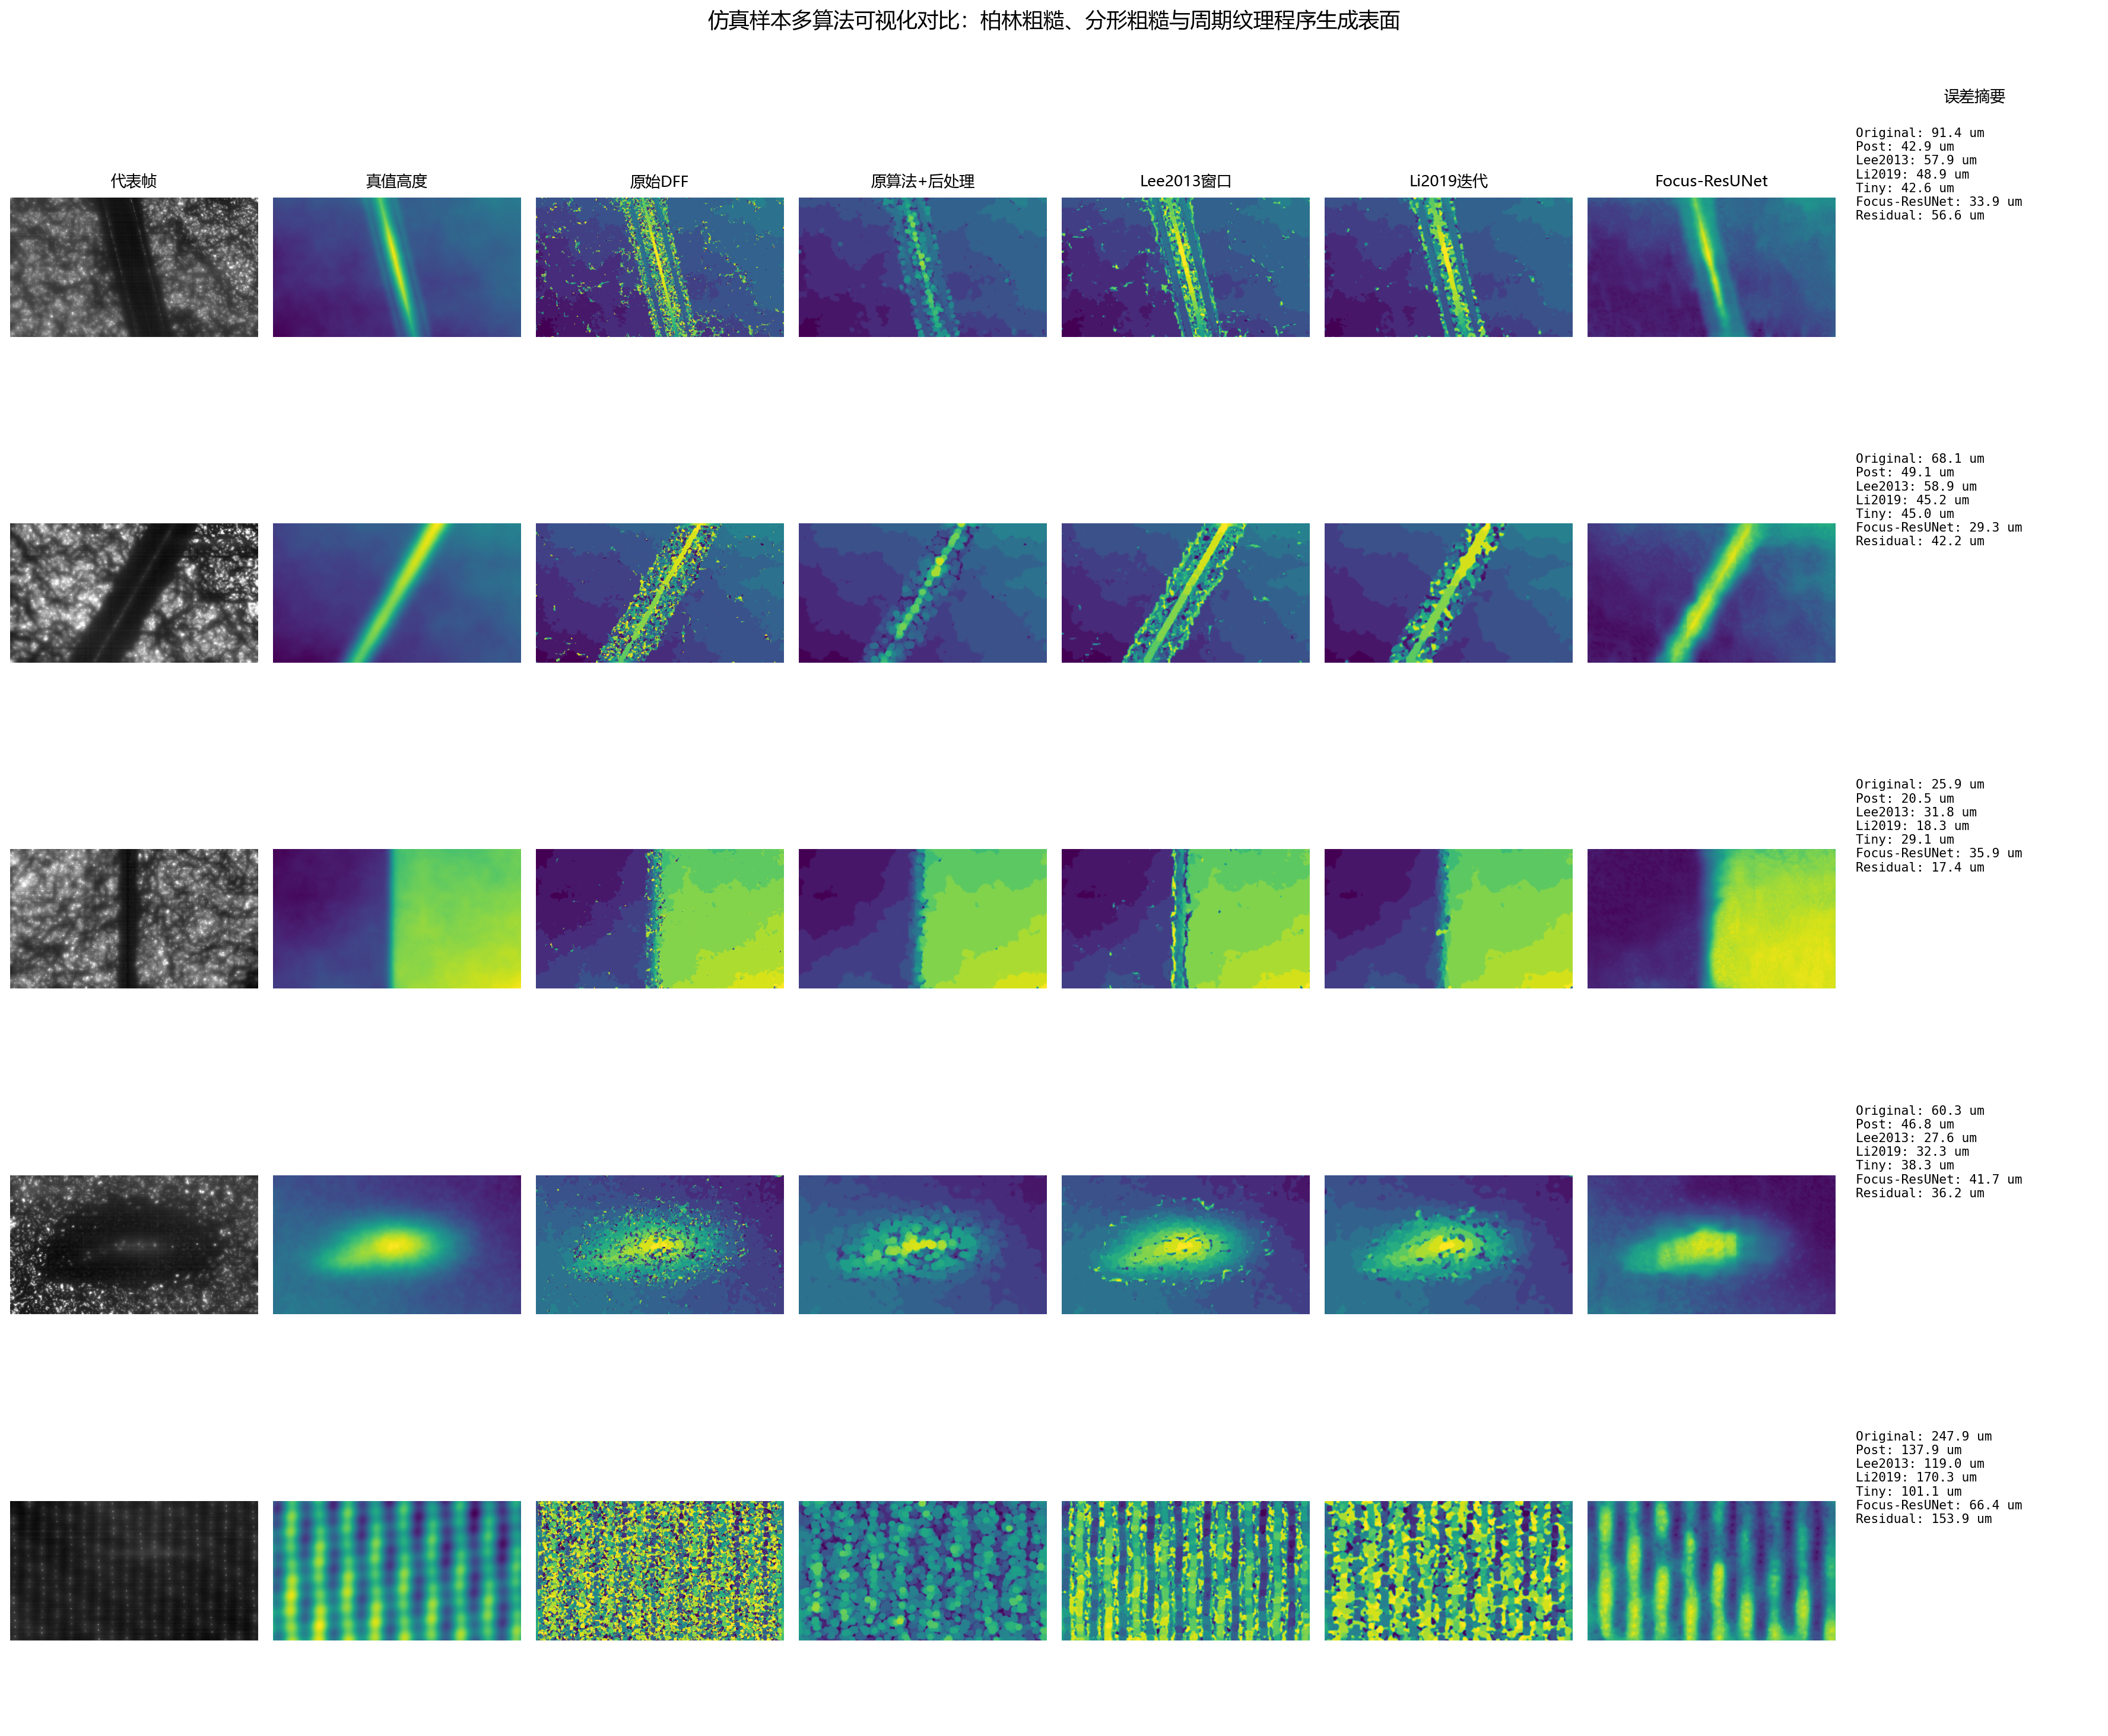
\includegraphics[width=\textwidth]{results/figures/simulation_multisample_algorithm_panel.png}
\caption{Two-dimensional height reconstruction comparison on representative synthetic samples. The panel compares ground truth, traditional DFF variants, adaptive traditional baselines and learning-based models.}
\label{fig:synthetic_panel}
\end{figure}

\subsection{P10 V-valley case study}

The P10 V-valley with rough wide bottom is the most important difficult case. It has a large height range, a wide valley, rough bottom texture and reflectance risk. Traditional DFF often selects incorrect focus layers at the valley bottom and along the valley edge.

\begin{table}[htbp]
\centering
\caption{Error metrics on the P10 V-valley sample.}
\small
\begin{tabular}{lccc}
\toprule
Method & P10 MAE & High-risk MAE & Edge MAE \\
 & \((\mu\mathrm{m})\) & \((\mu\mathrm{m})\) & \((\mu\mathrm{m})\) \\
\midrule
Original DFF & 160.17 & 39.23 & 270.77 \\
Original DFF + post & 120.87 & 29.31 & 227.46 \\
Lee2013 adaptive window & 102.60 & 32.77 & 192.92 \\
Li2019 adaptive iteration & 98.08 & \textbf{21.62} & 186.08 \\
GADFF & 167.46 & 39.23 & 282.00 \\
TinyDepthNet & 92.46 & 41.86 & 157.28 \\
Focus-ResUNet & \textbf{62.07} & 27.88 & \textbf{105.93} \\
PA-FRU & 101.57 & 26.15 & 178.44 \\
\bottomrule
\end{tabular}
\end{table}

Original DFF gives \(160.17~\mu\mathrm{m}\) MAE and \(270.77~\mu\mathrm{m}\) edge MAE, showing strong failure near the valley wall and rough bottom. Li2019 adaptive iteration improves MAE to \(98.08~\mu\mathrm{m}\) and achieves the best high-risk MAE, indicating that traditional iterative enhancement stabilizes some risky regions. Focus-ResUNet further reduces MAE to \(62.07~\mu\mathrm{m}\) and edge MAE to \(105.93~\mu\mathrm{m}\), making it the best overall method on this main case.

\begin{figure}[htbp]
\centering
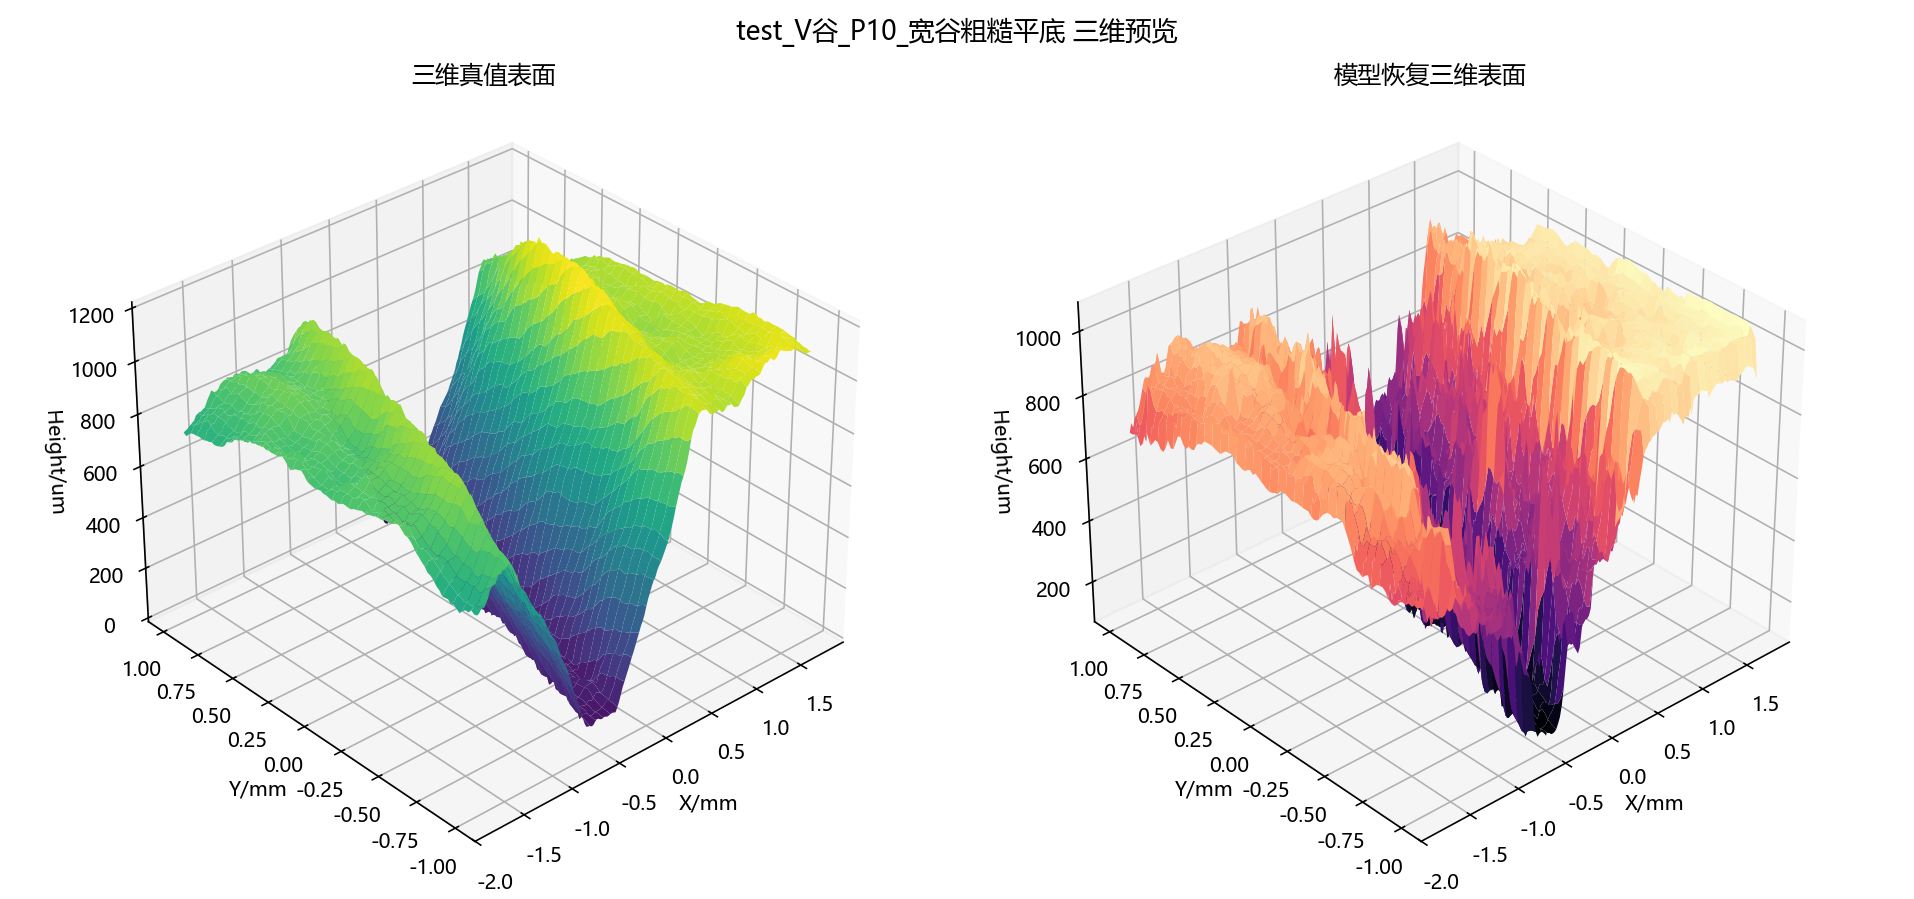
\includegraphics[width=0.92\textwidth]{assets/figures/readme_showcase/ppt_synthetic_surface_3d_comparison.png}
\caption{Three-dimensional synthetic surface comparison used for presentation and paper evidence. The result illustrates how learning-based correction improves the relative morphology of difficult synthetic surfaces.}
\label{fig:synthetic_3d}
\end{figure}

\subsection{Real-sample reconstruction}

Real-sample results are evaluated by visual stability and no-reference indicators because no external height truth is available. The average no-reference metrics are shown in Table~\ref{tab:real_metrics}.

\begin{table}[htbp]
\centering
\caption{No-reference stability metrics on real samples.}
\label{tab:real_metrics}
\small
\begin{tabular}{lcccc}
\toprule
Method & Roughness & Edge corr. & Rel. dynamic range & Low-conf. spikes \\
\midrule
Original DFF & 0.0977 & -0.0394 & 0.6964 & 9179.7 \\
Original DFF + post & 0.0130 & -0.0296 & 0.3944 & 4091.3 \\
GADFF & 0.0316 & -0.0295 & 0.5406 & 3351.4 \\
Lee2013 adaptive window & 0.0295 & -0.0209 & 0.6325 & 5018.7 \\
Li2019 adaptive iteration & 0.0318 & -0.0233 & 0.6515 & 5433.6 \\
TinyDepthNet & \textbf{0.0067} & -0.0243 & \textbf{0.3623} & 49.0 \\
Focus-ResUNet & 0.0078 & \textbf{0.0009} & 0.5317 & \textbf{2.0} \\
PA-FRU & 0.0594 & -0.0343 & 0.5203 & 9262.1 \\
\bottomrule
\end{tabular}
\end{table}

TinyDepthNet has the lowest roughness and a low spike count, giving the most natural and stable visual reconstruction among the tested methods. Focus-ResUNet has the best edge correlation and the lowest spike count, but its relative dynamic range is larger, and in visual inspection it is more likely to amplify real-sample reflectance and out-of-domain texture patterns. Therefore, TinyDepthNet is treated as the most robust current method for real-sample visualization.

This result differs from the synthetic ranking because the evaluation target changes. Synthetic samples have known height maps and evaluate absolute height error. Real samples lack ground truth and evaluate relative morphology stability. Real focus stacks contain illumination variation, sensor noise, local saturation, surface contamination and mechanical stepping errors that are not fully covered by the synthetic generator. A larger model can interpret these out-of-domain features as height variation, while TinyDepthNet's smaller capacity and smoother output provide practical regularization.

\begin{figure}[htbp]
\centering
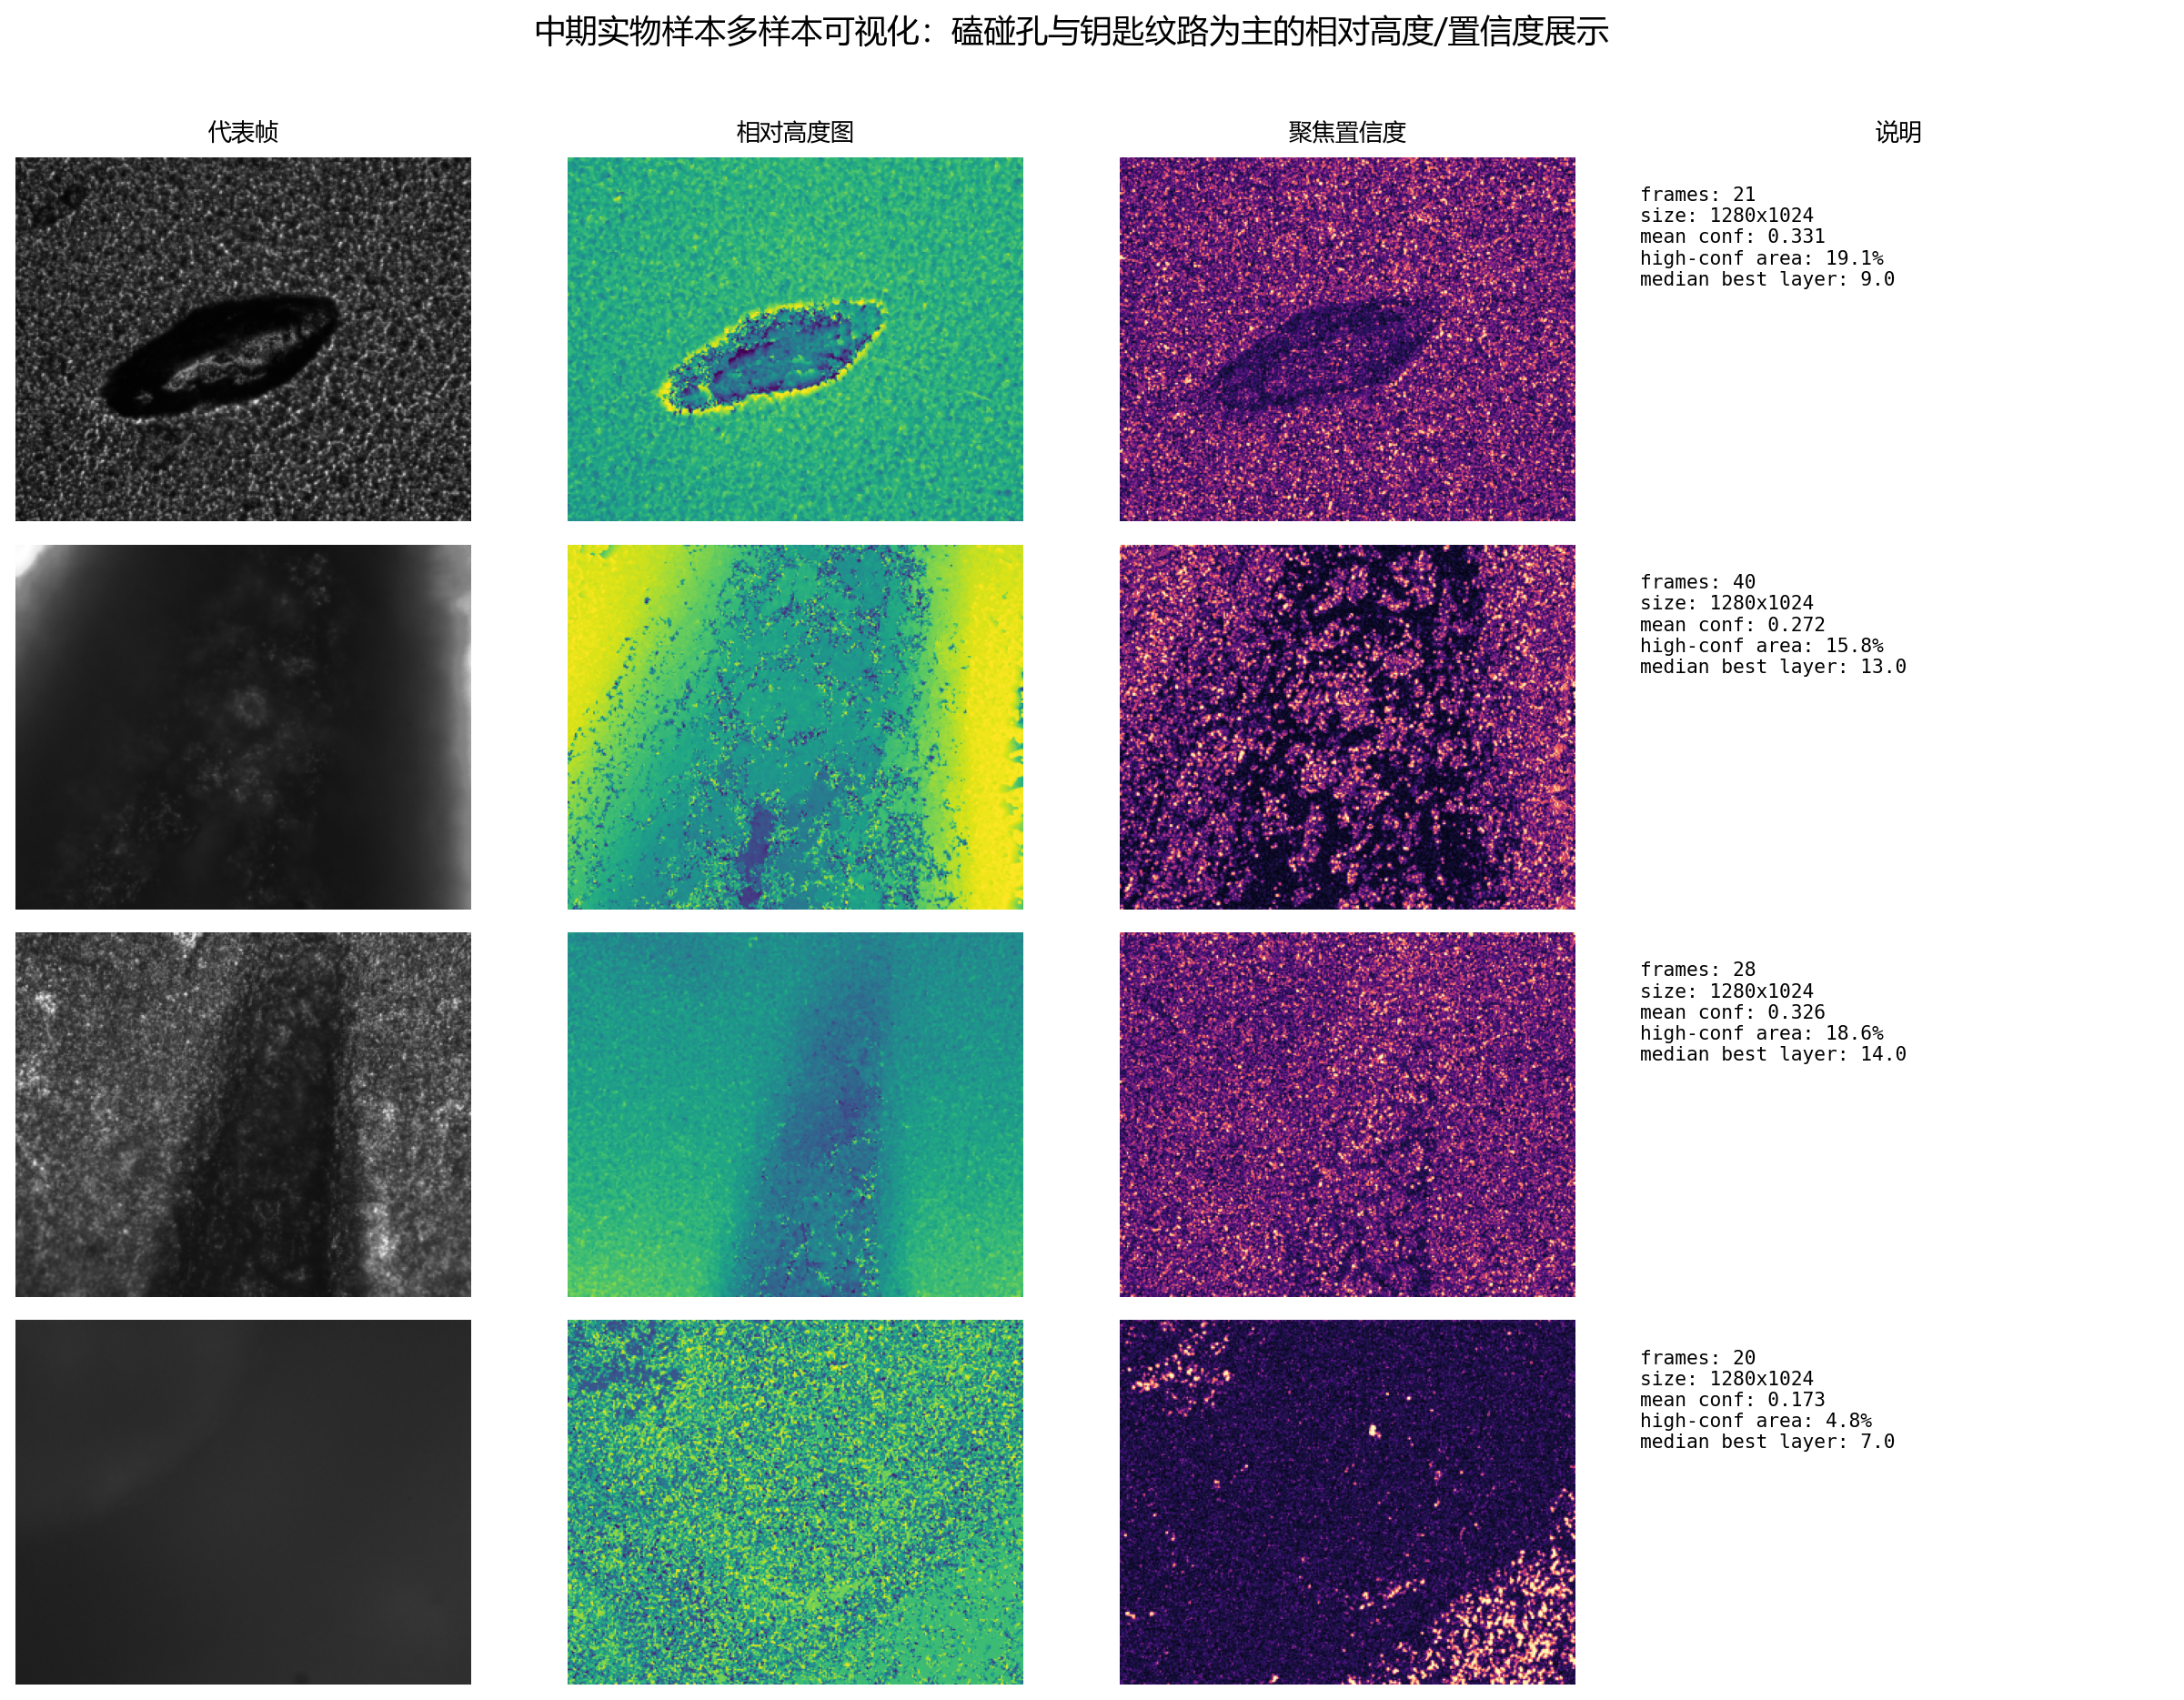
\includegraphics[width=\textwidth]{results/figures/real_midterm_multisample_panel.png}
\caption{Real-sample relative height and focus-confidence visualization. These samples are used for engineering verification and relative morphology analysis because no calibrated height ground truth is available.}
\label{fig:real_panel}
\end{figure}

\begin{figure}[htbp]
\centering
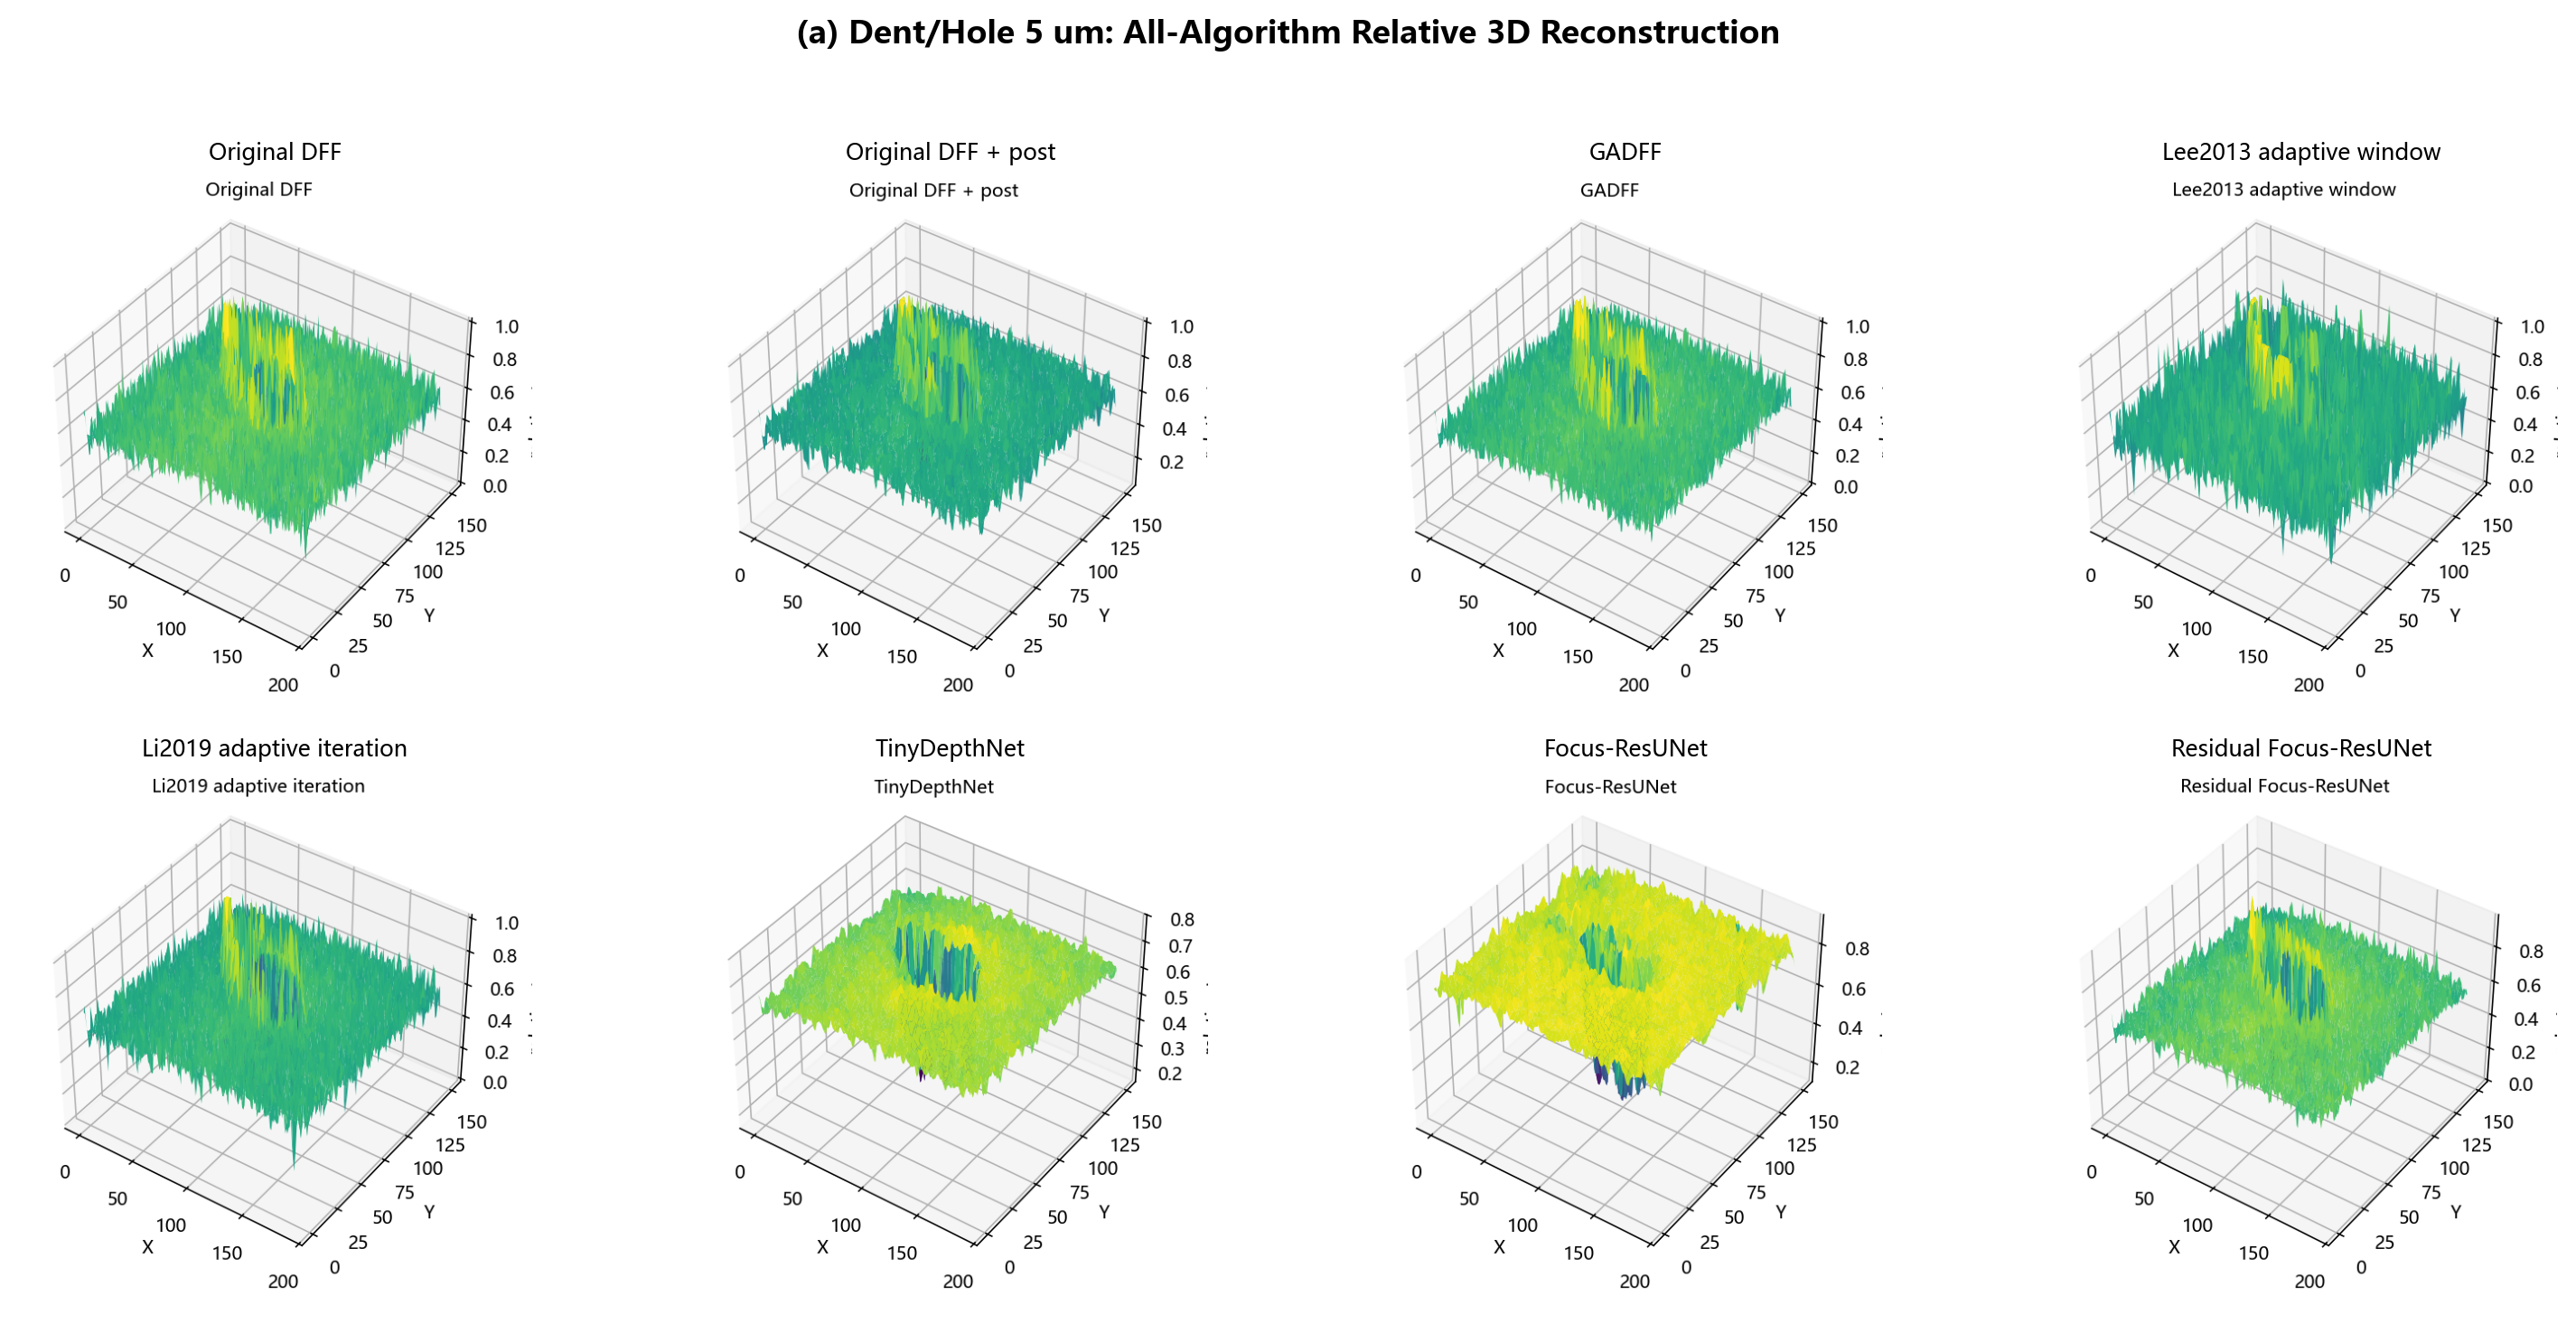
\includegraphics[width=0.92\textwidth]{assets/figures/readme_showcase/real_pit_5um_all_algorithm_3d.png}
\caption{Three-dimensional reconstruction comparison for a real dent or pit sample. The figure highlights the difference between traditional DFF variants and learning-based correction models under reflective real-sample conditions.}
\label{fig:real_pit_3d}
\end{figure}

\begin{figure}[htbp]
\centering
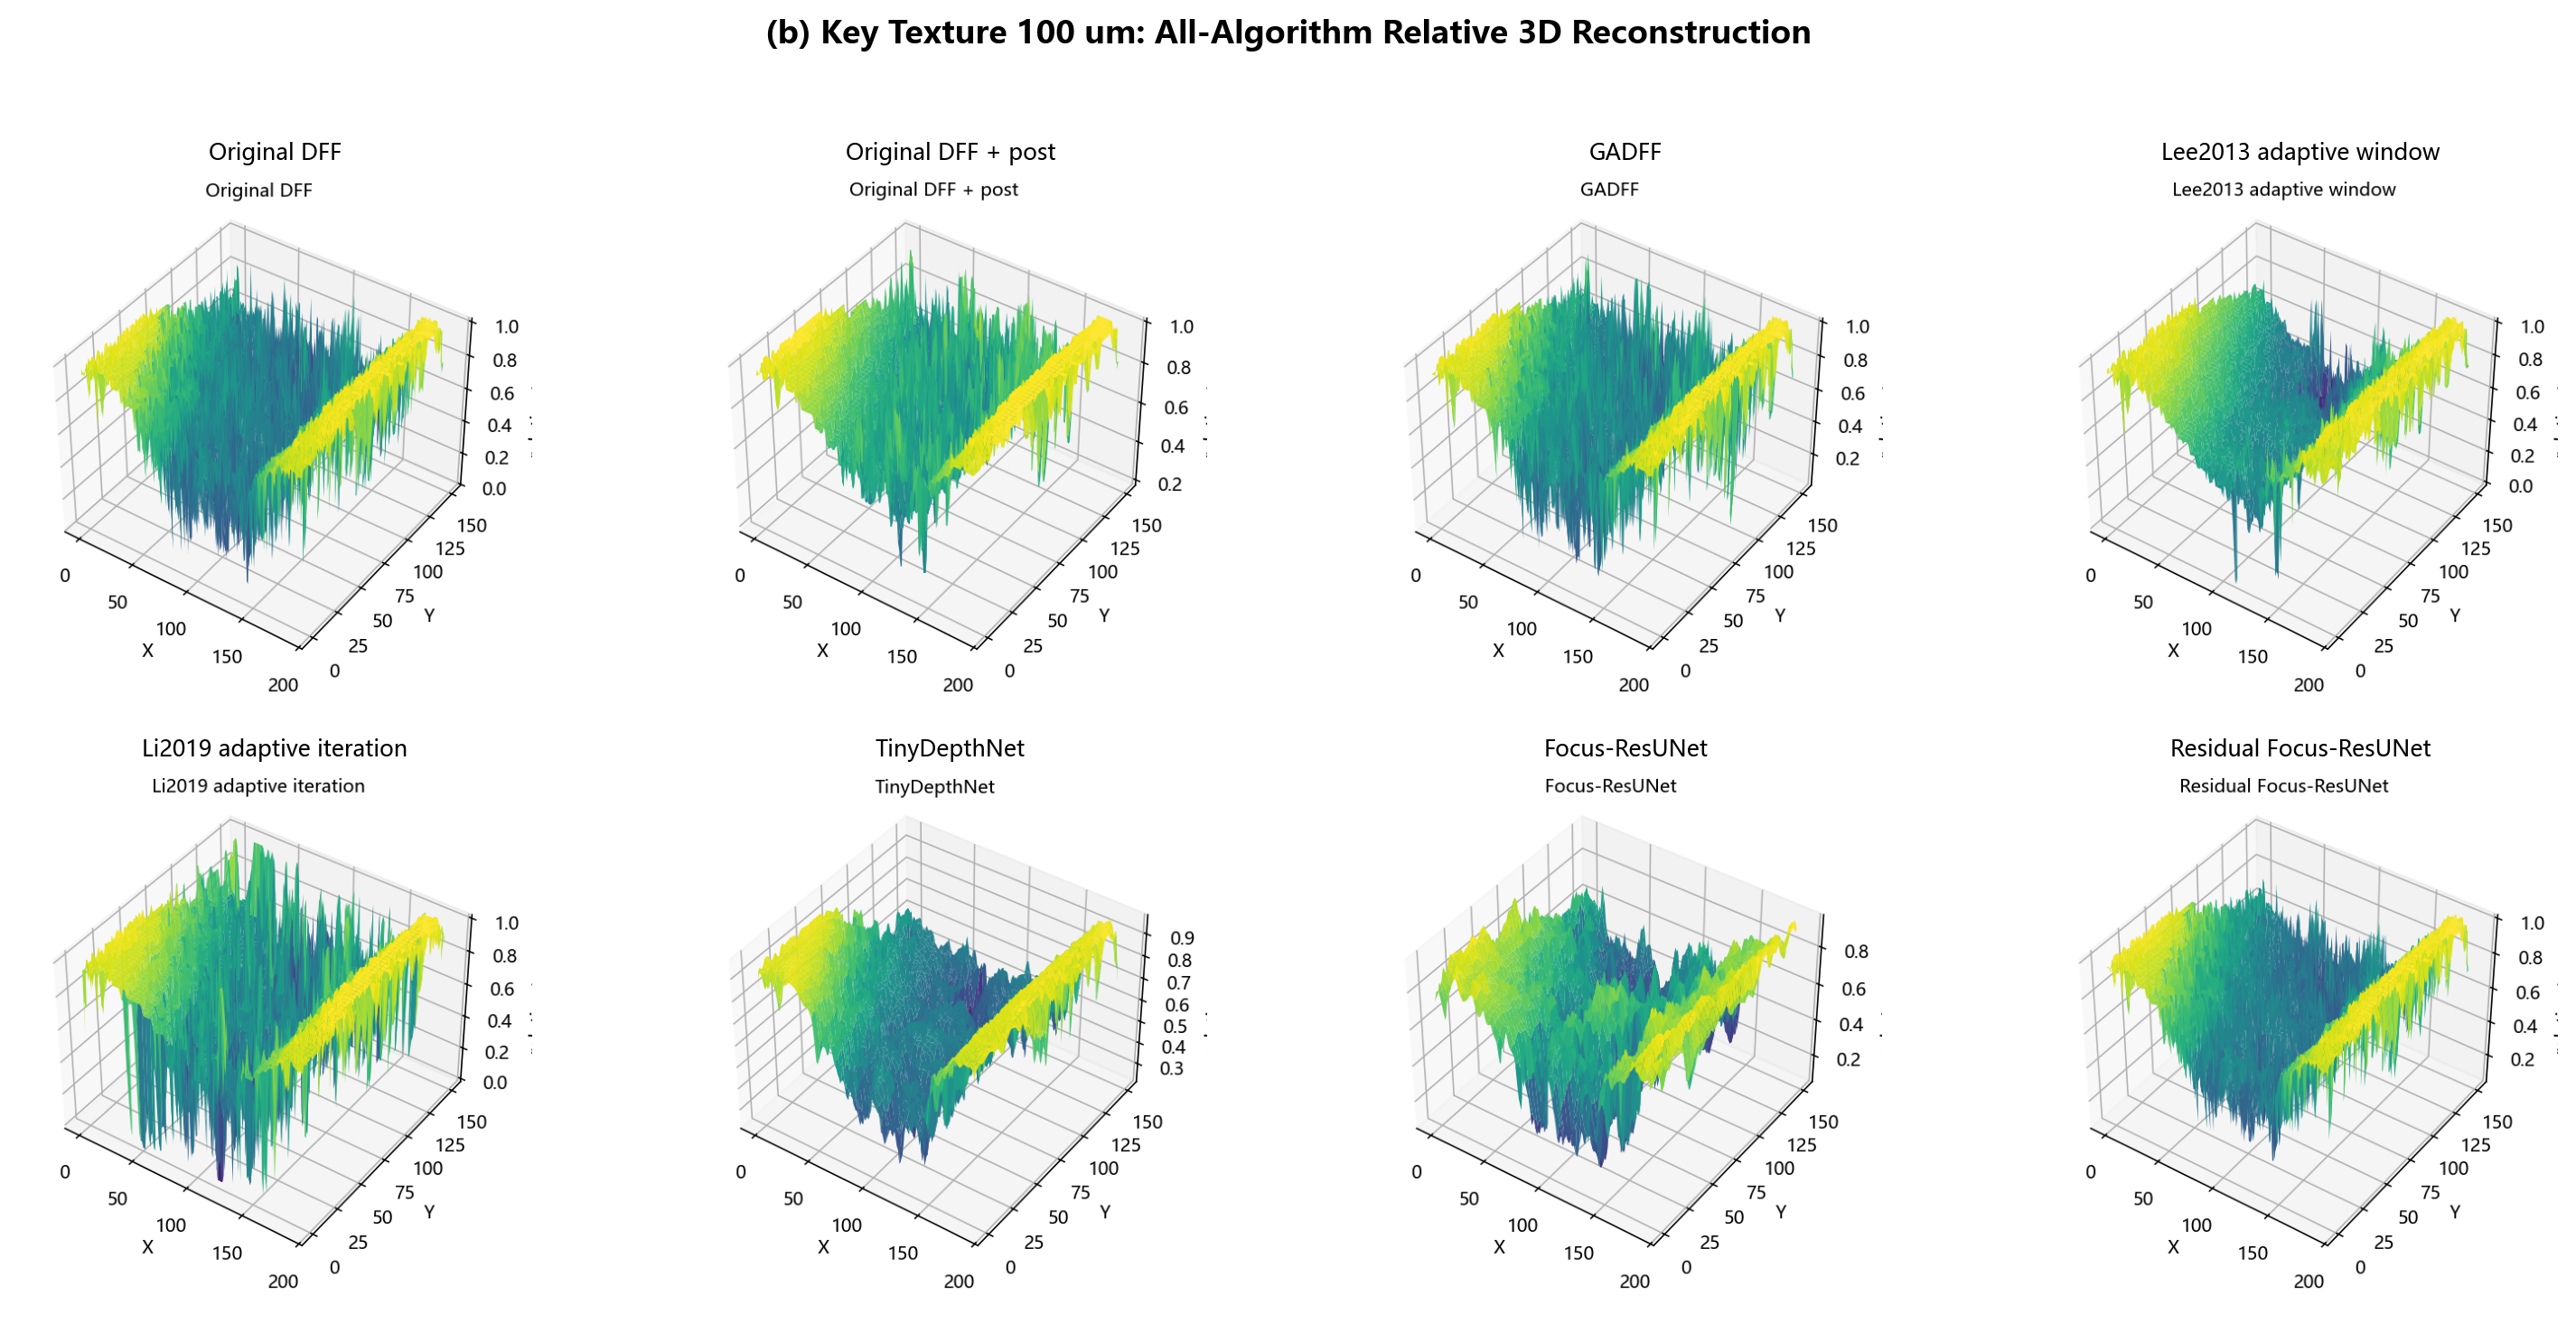
\includegraphics[width=0.92\textwidth]{assets/figures/readme_showcase/real_key_texture_100um_all_algorithm_3d.png}
\caption{Three-dimensional reconstruction comparison for a real key-texture sample. Dense directional texture and local highlights make this sample useful for evaluating visual stability.}
\label{fig:real_key_texture_3d}
\end{figure}

\begin{figure}[htbp]
\centering
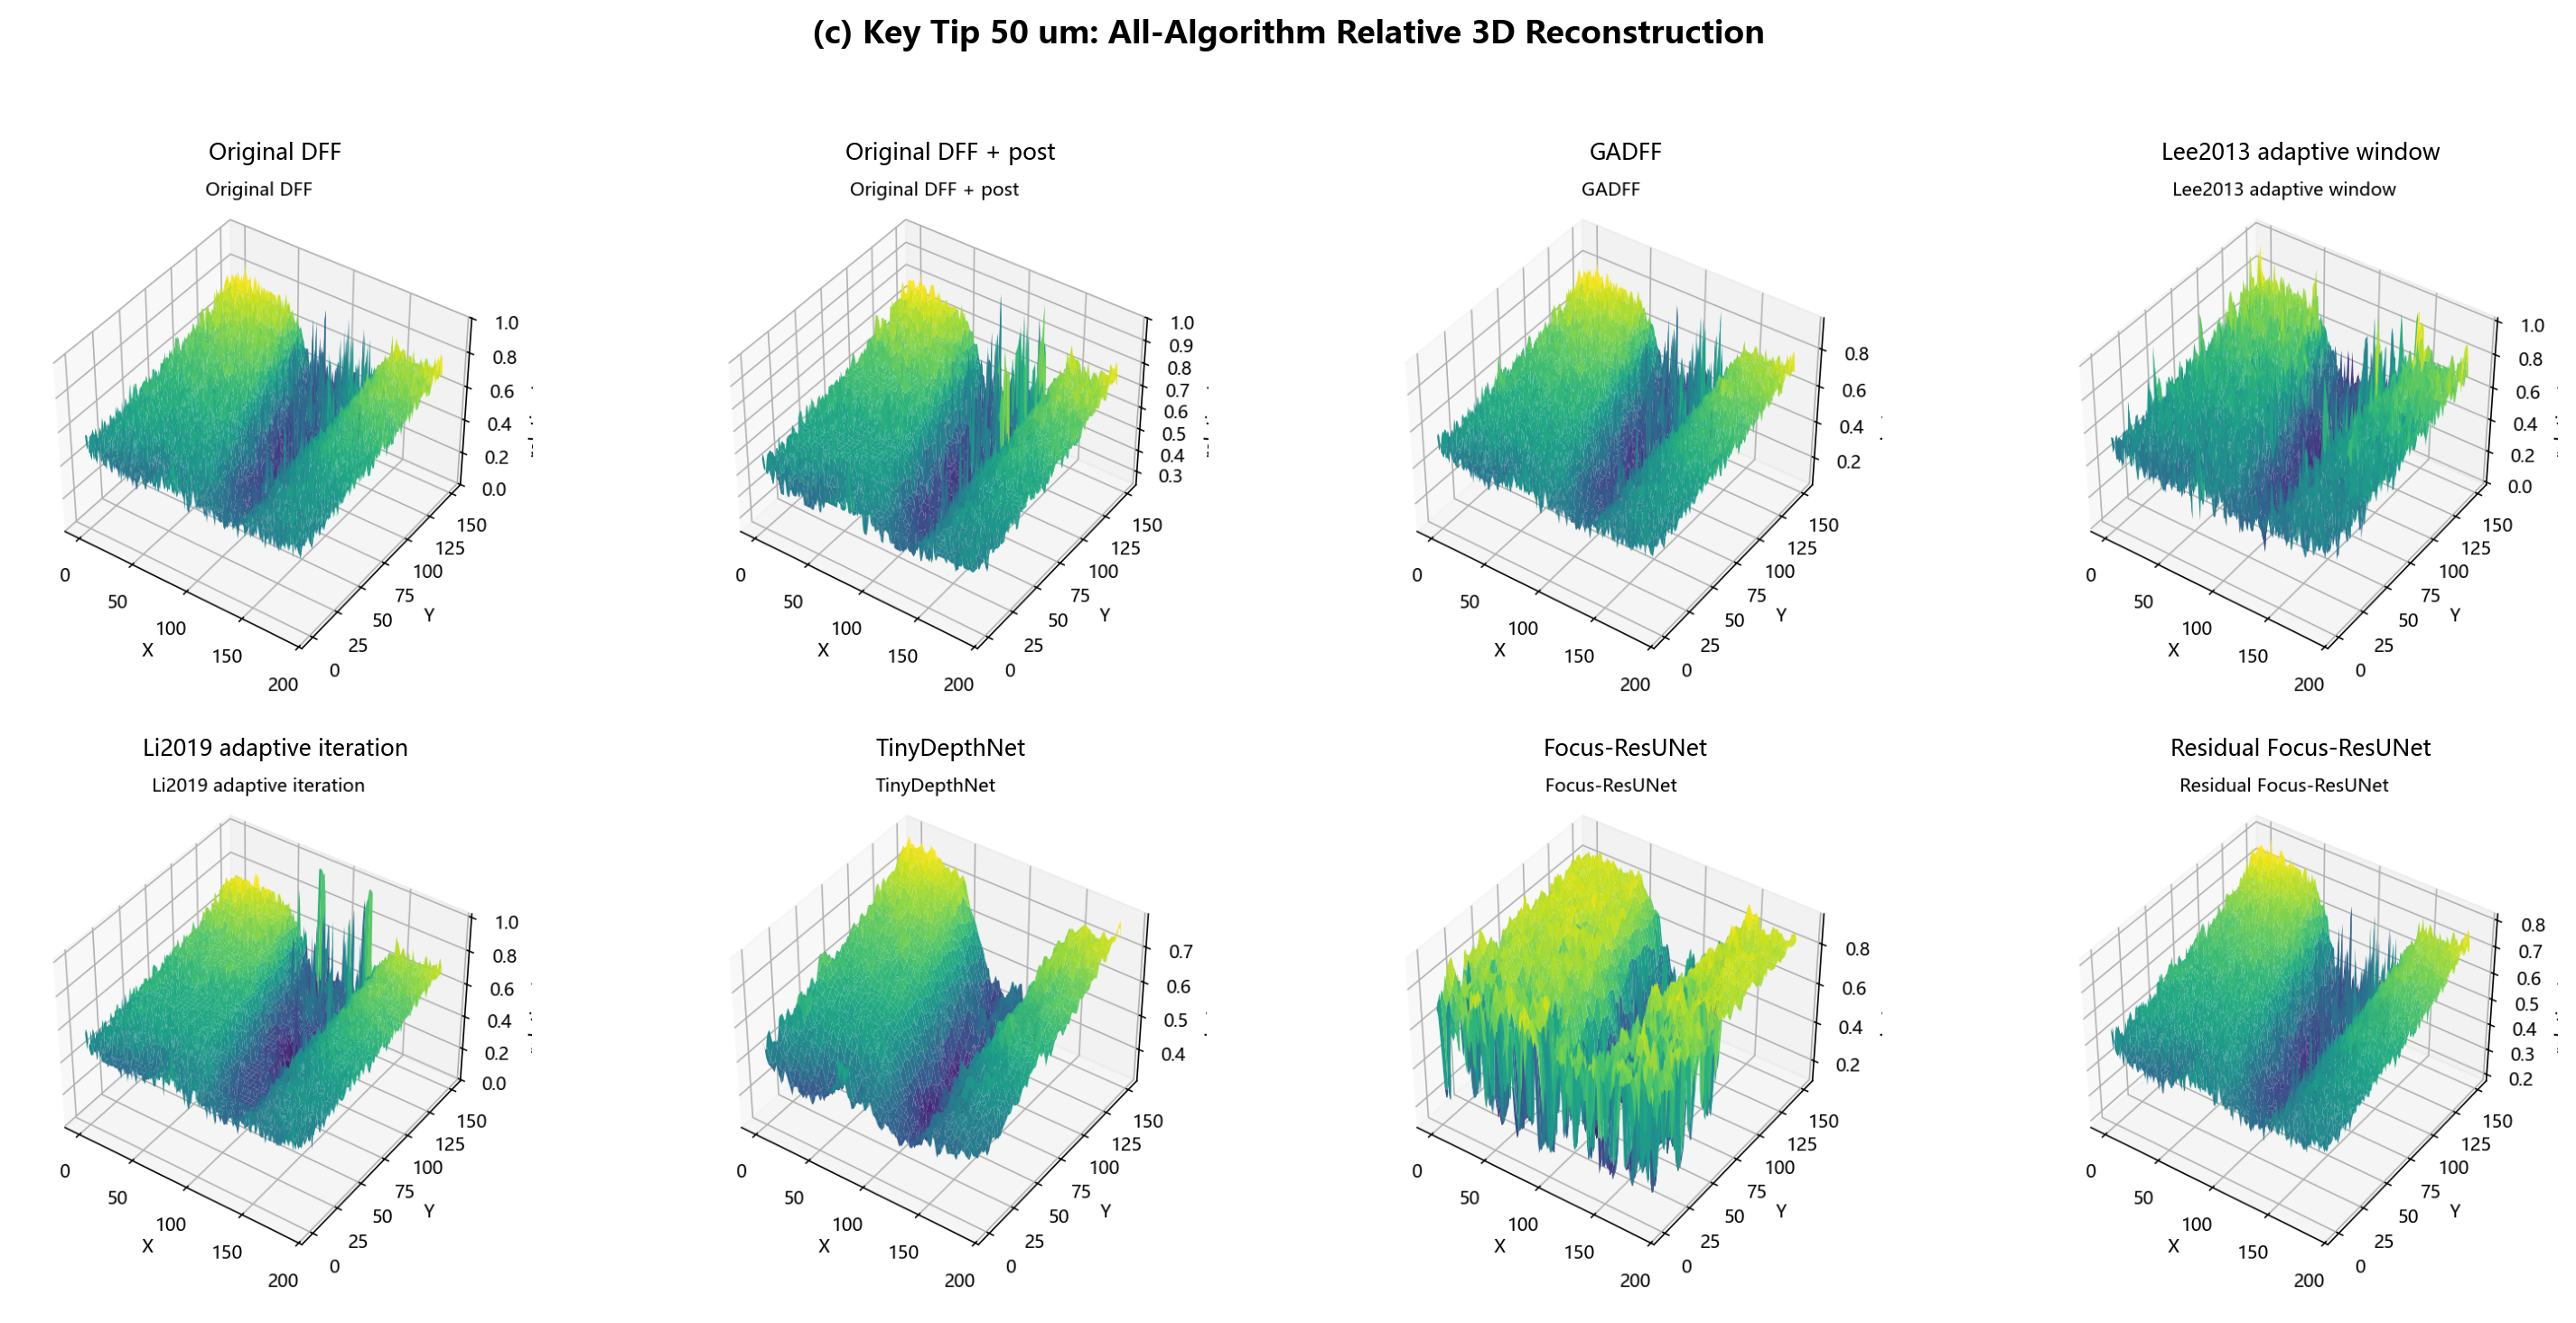
\includegraphics[width=0.92\textwidth]{assets/figures/readme_showcase/real_key_tip_50um_all_algorithm_3d.png}
\caption{Three-dimensional reconstruction comparison for a real key-tip sample. The sharp metallic edge tests reconstruction behavior near abrupt geometry and strong reflection.}
\label{fig:real_key_tip_3d}
\end{figure}

\section{Discussion}

The experiments show that traditional DFF remains an important engineering baseline. It is interpretable, training-free and directly applicable to real focus stacks. However, the synthetic results confirm that Original DFF is vulnerable to low texture, glare, periodic patterns and structural edges. Post-processing and adaptive windows reduce noise and improve stability, but they cannot fully resolve false focus peaks in difficult surfaces.

Focus-ResUNet performs best in synthetic quantitative validation because it uses the richest input: original focus-stack frames, focal-difference volume and prior maps. The focal-difference channels help the model observe focus-state changes along the optical axis, while DFF and GADFF priors give interpretable initial depth and risk information. This combination is especially useful in complex textures and strong-reflection conditions.

The real-sample results reveal the current domain gap. The synthetic generator includes simplified coaxial illumination, roughness-related specular highlights, bloom glare, low-frequency stray light, ghost flare and basic camera noise. These components are useful for controlled experiments, but they are not yet calibrated from real camera, lens and illumination parameters. Therefore, synthetic quantitative superiority does not automatically imply best real-sample visual stability. The current evidence supports a practical conclusion: Focus-ResUNet is the strongest model under synthetic ground-truth supervision, while TinyDepthNet is the most stable model for current real-sample relative visualization.

The unit boundary must also be kept clear. In synthetic samples, normalized height error can be converted to micrometer MAE because each sample has a known height range. In real samples, the output is normalized relative height. Without a calibrated mapping from focus layer to physical height, real-sample color maps and 3D surfaces should not be read as absolute micrometer measurements.

\section{Conclusion and Future Work}

This paper presents a complete comparison framework for focus-stack based relative 3D reconstruction of multi-material surface defects. The framework covers traditional DFF, post-processing, glare-aware prior modeling, adaptive traditional baselines and learning-based correction models. A synthetic dataset with known height maps provides quantitative evidence, and real focus-stack samples provide engineering verification and visual stability analysis.

On seven synthetic test samples, Focus-ResUNet achieves the best average MAE of \(53.22~\mu\mathrm{m}\), compared with \(100.55~\mu\mathrm{m}\) for Original DFF and \(57.31~\mu\mathrm{m}\) for TinyDepthNet. On the P10 V-valley case, it reduces MAE to \(62.07~\mu\mathrm{m}\) and greatly improves edge-region error. These results demonstrate that focal-difference features and DFF/GADFF priors can help neural models correct traditional focus-stack reconstruction errors.

On real samples, TinyDepthNet gives the most stable current visualization, with the lowest roughness and far fewer low-confidence spikes than traditional methods. This result indicates that real focus-stack reconstruction should consider not only supervised error correction under ground truth but also robustness to uncalibrated imaging conditions.

The main limitations are clear. First, real samples lack external height ground truth, so real-sample absolute accuracy cannot be reported. Second, the synthetic imaging model is still simplified and not calibrated with real optical system parameters. Third, learning-based models show a domain gap between synthetic training and real imaging. Future work should collect real calibrated height data using profilometry, confocal microscopy, white-light interferometry or standard step samples; expand material and defect categories; apply domain randomization or domain adaptation; and design structure-aware gating strategies that preserve DFF priors in reliable regions and enable learning-based correction in glare, low-texture and complex-texture regions.

\begin{thebibliography}{12}

\bibitem{nayar1994shape}
Nayar, S. K., and Nakagawa, Y. (1994). Shape from focus. \textit{IEEE Transactions on Pattern Analysis and Machine Intelligence}, 16(8), 824--831.

\bibitem{pertuz2013analysis}
Pertuz, S., Puig, D., and Garcia, M. A. (2013). Analysis of focus measure operators for shape-from-focus. \textit{Pattern Recognition}, 46(5), 1415--1432.

\bibitem{lee2013adaptive}
Lee, I., Mahmood, M. T., and Choi, T.-S. (2013). Adaptive window selection for 3D shape recovery from image focus. \textit{Optics \& Laser Technology}, 45, 21--31.

\bibitem{li2019adaptive}
Li, L., Pan, Z., Cui, H., Liu, J., Yang, S., Liu, L., Tian, Y., and Wang, W. (2019). Adaptive window iteration algorithm for enhancing 3D shape recovery from image focus. \textit{Chinese Optics Letters}, 17(6), 061001.

\bibitem{yang2022deep}
Yang, F., Huang, X., and Zhou, Z. (2022). Deep Depth from Focus with Differential Focus Volume. \textit{Proceedings of the IEEE/CVF Conference on Computer Vision and Pattern Recognition}, 12642--12651.

\bibitem{ronneberger2015unet}
Ronneberger, O., Fischer, P., and Brox, T. (2015). U-Net: Convolutional Networks for Biomedical Image Segmentation. \textit{MICCAI 2015}, 234--241.

\bibitem{he2016deep}
He, K., Zhang, X., Ren, S., and Sun, J. (2016). Deep Residual Learning for Image Recognition. \textit{Proceedings of the IEEE Conference on Computer Vision and Pattern Recognition}, 770--778.

\bibitem{wu2018group}
Wu, Y., and He, K. (2018). Group Normalization. \textit{ECCV 2018}, 3--19.

\bibitem{huber1964robust}
Huber, P. J. (1964). Robust Estimation of a Location Parameter. \textit{The Annals of Mathematical Statistics}, 35(1), 73--101.

\bibitem{charbonnier1994two}
Charbonnier, P., Blanc-Feraud, L., Aubert, G., and Barlaud, M. (1994). Two Deterministic Half-Quadratic Regularization Algorithms for Computed Imaging. \textit{IEEE International Conference on Image Processing}, 2, 168--172.

\bibitem{shang2021review}
Shang, M., and Yu, F. (2021). Research progress of zoom microscopy three-dimensional measurement systems. \textit{Laser \& Optoelectronics Progress}, 58(16), 1600002.

\bibitem{shi2019performance}
Shi, Y., Yin, Q., and Lu, R. (2019). Performance analysis of three-dimensional measurement algorithms for zoom microscopic imaging. \textit{Laser \& Optoelectronics Progress}, 56(7), 071202.

\end{thebibliography}

\end{document}
